\begin{figure}[t]
\centering
\resizebox{\columnwidth}{!}{%
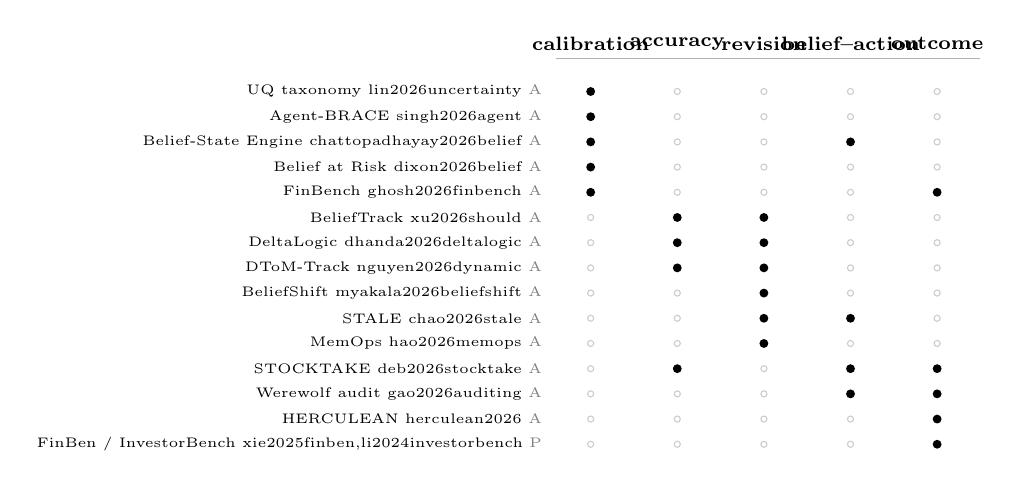
\begin{tikzpicture}[font=\scriptsize, x=11mm, y=3.2mm]
\foreach \c/\x in {calibration/1, accuracy/2, revision/3, belief--action/4, outcome/5} \node[align=center, font=\scriptsize\bfseries, rotate=0] at (\x,0.9) {\c};
\foreach \name/\ev/\y/\dots in {
  {UQ taxonomy \citep{lin2026uncertainty}}/A/-1/{1},
  {Agent-BRACE \citep{singh2026agent}}/A/-2/{1},
  {Belief-State Engine \citep{chattopadhayay2026belief}}/A/-3/{1,4},
  {Belief at Risk \citep{dixon2026belief}}/A/-4/{1},
  {FinBench \citep{ghosh2026finbench}}/A/-5/{1,5},
  {BeliefTrack \citep{xu2026should}}/A/-6/{2,3},
  {DeltaLogic \citep{dhanda2026deltalogic}}/A/-7/{2,3},
  {DToM-Track \citep{nguyen2026dynamic}}/A/-8/{2,3},
  {BeliefShift \citep{myakala2026beliefshift}}/A/-9/{3},
  {STALE \citep{chao2026stale}}/A/-10/{3,4},
  {MemOps \citep{hao2026memops}}/A/-11/{3},
  {STOCKTAKE \citep{deb2026stocktake}}/A/-12/{2,4,5},
  {Werewolf audit \citep{gao2026auditing}}/A/-13/{4,5},
  {HERCULEAN \citep{herculean2026}}/A/-14/{5},
  {FinBen / InvestorBench \citep{xie2025finben,li2024investorbench}}/P/-15/{5}}
 {\node[anchor=east, font=\tiny] at (0.55,\y) {\name~{\color{gray}\ev}};
  \foreach \x in {1,...,5} \draw[gray!40] (\x,\y) circle (1.1pt);
  \foreach \x in \dots \fill (\x,\y) circle (1.6pt);}
\draw[gray!60] (0.6,0.3) -- (5.5,0.3);
\end{tikzpicture}}
\caption{Which belief-level construct each evaluation paper reports. Filled dots mark a reported metric. \textsf{P} = peer-reviewed venue, \textsf{A} = arXiv preprint at the time of writing. No two papers report the same metric for the same construct, which is the fragmentation this section addresses.}
\label{fig:metrics}
\end{figure}
